\documentclass[11pt]{article}

\usepackage[T1]{fontenc}
\usepackage[utf8]{inputenc}
\IfFileExists{lmodern.sty}{\usepackage{lmodern}}{}
\usepackage[margin=1in]{geometry}
\usepackage{microtype}
\usepackage{amsmath}
\usepackage{graphicx}
\usepackage{booktabs}
\usepackage{tabularx}
\usepackage{array}
\usepackage{multirow}
\usepackage{enumitem}
\usepackage{xcolor}
\usepackage[numbers,sort&compress]{natbib}
\usepackage{xurl}
\usepackage[hidelinks]{hyperref}
\emergencystretch=2em
\usepackage{caption}
\captionsetup{font=small,labelfont=bf}
\setlist{itemsep=2pt,topsep=4pt}
\newcolumntype{L}{>{\raggedright\arraybackslash}X}
\newcommand{\lbl}[1]{\textsf{[#1]}}
\newcommand{\todo}[1]{\textcolor{red}{[TODO: #1]}}
\renewcommand{\bibfont}{\small}

\title{Does an LLM Village Retrace Human History?\\[2pt]
\large A 108-Year Observational Study of an LLM-Agent Society Advanced Through\\ a Planned Prehistory-to-State Sequence}
\author{Ryo Tanohata\\ Independent researcher\\ \texttt{\todo{email}}}
\date{Draft, 29 October 2026}

\begin{document}
\maketitle

\begin{abstract}
We report an observational study of a single, long-running simulation in which a village of large-language-model (LLM) agents lived on a simulated river valley for 108 simulated years (13{,}079 simulated days; one simulated year is 120 days). The adults were role-played by Claude models (Haiku in early phases; from simulated year 62, household representatives by Sonnet with about one in eight by Opus, and non-representatives' feelings by Haiku). The designer advanced the society through planned phases modelled on the West Asian sequence: a hunter-gatherer phase (F1--F6) and an agrarian phase (G1--G9: village and fields, livestock, pottery and storage, household property, leaders and festivals, trade/towns/records, state formation, external pressure, long-distance trade). No new simulation was run for this paper; we compare the existing records with the archaeological sequence by \emph{ordering} and \emph{conditions}, not durations. Three findings stand out. (1) The order of subsistence technologies (settlement, cultivation, fields, goats, sickles, pottery, household storage, inheritance) broadly matched the West Asian order, with notable inversions (pottery before family houses and stores; fire very late), whereas institutions stalled: taxation, enforced written law, officials, rulers, war, towns and writing never emerged in the village. (2) Technology acted as a \emph{floor} rather than an engine: most technologies were opened by the designer's phase gates, they raised food security (e.g.\ pest losses fell to zero after pottery), and the household-storage gate coincided with a jump in the wealth Gini from 0 to 0.84; clay-tablet records were used for dispute bookkeeping but never for taxation and stopped when the record-keepers died. (3) Behaviour mixed human-like patterns (festival reconciliation, closing to outsiders in hard years, refusing tribute ``for the children'') with patterns better described as LLM-like: after simulated year 50, zero restitution verdicts among 263 dispute settlements, zero homicide or war, a large gap between sharing talk and sharing acts (0 of 1{,}134 opportunities to release household stores), and behaviour that split by model rather than by person. Rule-based and scenario experiments indicate that the missing tax-and-record institutions were not blocked by the simulation mechanics but by the choices of the LLM representatives. Because this is one run with designer interventions, rewinds and a mid-run model switch, all results are case observations, not general laws.
\end{abstract}

\section{Introduction}

LLM agents are increasingly used to build artificial societies \citep{park2023generative,altera2024sid,piatti2024cooperate} and to stand in for human participants in social-science experiments \citep{horton2023homo,aher2023using,argyle2023out}. A natural but rarely tested question follows: if an LLM-agent society is walked through the material conditions of human prehistory, does it reproduce the \emph{sequence} of human history, and where it does not, why not?

This paper is an observational study of one such society. Beginning in late September 2026, a five-person band of LLM agents was placed on a simulated river valley. Over about one month of wall-clock time and 108 simulated years, the designer (the author, working with Claude Code) advanced the society through planned phases that follow the textbook West Asian sequence from mobile foraging to state formation and long-distance trade. Agents decided their work, speech, sharing, proposals and votes once per season; a deterministic world model computed food, births, deaths, disputes and regional politics day by day. At the time of writing the run is paused at the end of simulated year 108 (day 13{,}079), in phase G9.

We ask three questions, posed by the author during the run:
\begin{enumerate}
  \item \textbf{Same and different:} Where does the village's trajectory match the archaeological sequence, where does it diverge, and what causes the divergences?
  \item \textbf{Technology:} What role did technology play in this society?
  \item \textbf{Humanness:} Which behaviours look human, which look like artefacts of the LLMs, and how could the two be told apart?
\end{enumerate}

\paragraph{Contributions.}
\begin{itemize}
  \item A long-horizon case record (108 simulated years, about 1.1 million logged events, 5{,}713 seasonal agent answers in the agrarian phase) of an LLM-agent society advanced through a planned prehistory-to-state sequence, with code, prompts, answers and state history publicly available.
  \item A comparison method that compares \emph{ordering and conditions} rather than durations, labels every claim by its epistemic status, and separates three causes of divergence: designer choices, world-model parameters, and LLM choice tendencies.
  \item Evidence, from the main run plus three side experiments (rule-based regional and village models, and a fixed-vignette probe of three Claude models), that the absence of state institutions in this village is attributable mainly to the LLM representatives' choices rather than to mechanical impossibility.
  \item A set of observations on ``humanness'' (forgiveness lock-in, talk--act gaps, model-dependent behaviour, absence of violence) and proposed criteria for distinguishing human-like from LLM-like behaviour, which motivate a planned, pre-registered follow-up study.
\end{itemize}

We stress at the outset what this paper is \emph{not}: it is not a test of any theory of state formation, it does not run new simulations, and it does not compare against human participants. It documents one run carefully and honestly so that its observations can be scrutinised and built upon.

\section{Related work}

\paragraph{LLM-agent societies.}
Generative Agents \citep{park2023generative} showed that LLM-driven characters with memory and reflection produce believable individual and small-group behaviour in a sandbox town over simulated days. Project Sid \citep{altera2024sid} scaled agent societies to hundreds or more agents in Minecraft and reported specialisation, collective rule change and cultural transmission. GovSim \citep{piatti2024cooperate} studied whether LLM agents sustain a common-pool resource and found that most models failed to reach sustainable equilibria. Our study differs in time horizon (a century of simulated time with births, deaths and inheritance), in the explicit use of a planned historical phase sequence as a yardstick, and in its focus on institutional emergence under a deterministic world model.

\paragraph{LLMs as simulated human subjects.}
Horton \citep{horton2023homo} proposed treating LLMs as ``homo silicus'' to replicate behavioural-economics experiments; Aher et al.\ \citep{aher2023using} introduced ``Turing experiments'' replicating classic studies with simulated participants; Argyle et al.\ \citep{argyle2023out} argued for ``algorithmic fidelity'' when conditioning on demographic backstories. Mei et al.\ \citep{mei2024turing} found that chatbot behaviour in trust, fairness and cooperation games is often within the human range but, where it differs, lies on the more altruistic and cooperative side; Akata et al.\ \citep{akata2025repeated} studied LLMs in repeated games. Sharma et al.\ \citep{sharma2024sycophancy} documented sycophancy in assistants trained with human feedback. These works motivate our interpretation that some of the village's ``kindness'' may be a property of the models rather than of the simulated situation.

\paragraph{State formation and egalitarianism.}
Carneiro's circumscription theory \citep{carneiro1970theory} links state formation to warfare under environmental or social circumscription; Turchin et al.\ \citep{turchin2013war} model the spread of large polities through inter-societal warfare. Scott \citep{scott2017against} emphasises that legible, storable grain made early states possible and that people often fled them. Graeber and Wengrow \citep{graeber2021dawn} argue that early societies moved between hierarchical and egalitarian arrangements by choice, and Boehm \citep{boehm1999hierarchy} describes active levelling of would-be dominants in egalitarian groups. Johnson's scalar-stress model \citep{johnson1982scalar} explains why growing groups adopt sequential (consensus-based) or simultaneous (ranked) hierarchies. Hirschman's exit/voice framework \citep{hirschman1970exit} is relevant to the village's responses to decline.

\paragraph{Storage, inequality and records.}
Flannery \citep{flannery2002origins} traced the shift from communal to private household storage in early villages. Kohler et al.\ \citep{kohler2017greater} measured house-size Gini coefficients across the Neolithic and later, and Bogaard et al.\ \citep{bogaard2019farming} linked large, durable wealth inequality to land-limited farming. On records, Schmandt-Besserat \citep{schmandt1992before} argued that writing grew out of token-based counting, and Englund \citep{englund2011accounting} showed that proto-cuneiform was overwhelmingly administrative bookkeeping. Henrich et al.\ \citep{henrich2005economic} provide cross-cultural human baselines for economic games in fifteen small-scale societies; we cite them as the type of human data a future yardstick should use.

\section{The simulation}
\label{sec:sim}

\subsection{World}
The world is a grid model of a river valley with forest, grassland, hills and a river. It contains wild plants (nuts, tubers, grass seed), small and large game, fish, a predator, seasons (30 days each, four per year), weather, food spoilage, pests, illness, births and deaths. From phase G1 onwards it also contains fields, goats, pottery, sickles, family houses, household stores, inheritance, disputes and their settlement, festivals, leaders, seals, counting tokens, envelopes and clay tablets, other settlements, exchange and loans, and (from G7) a regional model of neighbouring settlements that may demand tribute, form tiered polities, or fight. Food is tracked in physical units (handfuls of nuts or seed, pieces of meat) and converted to energy internally; agents never see kilocalories. The world model is written in Python (\texttt{sim/society/world.py}, \texttt{era2.py}, \texttt{g7.py}, \texttt{g9.py}, \texttt{region.py}, \texttt{hints.py}, \texttt{step.py}).

\subsection{Agents and prompts}
Each adult (age $\ge 15$) is an agent with a name, sex, age, personality (cooperation, boldness, curiosity, sociability on $[0,1]$), skills, hunger, fatigue, injuries, possessions, trust in others, and a free-text memory. Children do not answer; they eat from the village store and grow up in simulated time (one year of age per simulated year).

Each answer is produced by a separate model call. The workflow (\path{sim/society/tools/society2_seasons_workflow.js}) starts one sub-agent per adult; the sub-agent reads a prompt file, role-plays the character and writes a JSON answer file; a script then advances the world (\texttt{step.py season}) and commits the data to git. Prompts are in Japanese. They begin by instructing the agent that it has no knowledge of the outside world (``real place names, countries, history, religion, kings, money'') and should reason only from what it has experienced, heard or remembers. They then describe the agent, the village, the previous season's events, recent conversations, family, memories, the current laws (with vote history), the remembered year names, disputes and festivals, other villages, records, and the mechanics of every available action in plain language. Late in the run a representative's prompt is about 97\,KB long. The answer schema includes speech, a main job and place for the season, sowing/harvesting/picking/planting amounts, goats to slaughter, family members' jobs, whether to keep a household store, festival, leader choice, sealing, demands on neighbours, sharing from the household store, tribute responses, knowledge updates, a law proposal (optionally with penalty or tax) and votes on proposed laws.

When the number of adults exceeded 12, decisions passed to \emph{household representatives} (the eldest adult in each household); other adults answered only a short ``feeling and one sentence''. From phase G7 the village answered in ``year mode'': representatives met at a yearly meeting (summer), at an autumn meeting (from simulated year 62), at emergency re-meetings when the village store ran out, and in selected ``zoom'' seasons; in other seasons the yearly plan was executed.

\subsection{Models}
\begin{itemize}
  \item \textbf{Society 1.0 (F1--F6) and Society 2.0 up to day 7{,}438:} adults were role-played by Claude \textbf{Haiku} (one sub-agent call per adult per decision).
  \item \textbf{From day 7{,}439 (simulated year 62):} household representatives and leaders by Claude \textbf{Sonnet}, except that about one in eight representatives was assigned Claude \textbf{Opus} by a deterministic hash of the name (FNV-1a mod 8 $=0$; the same person always used the same model). Neighbouring settlements' councils used Sonnet; non-representatives' feelings used Haiku; the command-running helper used Haiku.
\end{itemize}
The workflow selected models by family alias (\texttt{haiku}, \texttt{sonnet}, \texttt{opus}); the exact model versions behind the aliases were not recorded per call \todo{author: confirm model versions used during 2026-09-30 to 2026-10-29}. Models used from day 7{,}439 are recorded per answer directory in \texttt{models.json}.

\subsection{Phases and gates}
The run followed a phase plan written before each part (Table~\ref{tab:phases}). Each phase had an entry condition evaluated at the end of each season. Many mechanics (e.g.\ pottery, family houses, household stores, seals) were enabled only when the corresponding phase was entered; we call these \emph{phase gates}. Some phases were closed by the author's decision when their conditions had not been met (G6, G7, G8). G7 introduced three state-formation conditions: (c1) the village belongs to a polity with three or more decision tiers, (c2) a fixed levy recorded on clay tablets for two consecutive years, (c3) a dispute judged under a written law with a penalty or conversion that was actually paid.

\begin{table}[t]
\centering\small
\caption{Planned phases and when the village entered them (simulated day; year = day/120). ``Gate'': mechanics opened on entry. Sources: \texttt{docs/society\_phase/*.md}, \texttt{docs/society2\_phase\_plan.md}.}
\label{tab:phases}
\begin{tabularx}{\linewidth}{@{}l l L r@{}}
\toprule
Phase & Model period (West Asia) & Content and outcome in the run & Entered (day) \\
\midrule
F1--F6 & Late Palaeolithic to PPNA & Foraging, broad-spectrum diet, storage, settlement, cultivation of wild plants; reached F6 (dependence on cultivated food) & 0--489 \\
G1 & Natufian/PPNA & Village grows (births, newcomers) & 489 \\
G2 & PPNB & Fields and goats & 1{,}229 \\
G3 & Pottery Neolithic & Surplus and craft; \emph{gate:} pottery, sickles, family houses, pests & 1{,}529 \\
G4 & Sabi Abyad & Household property, inheritance; \emph{gate:} household stores & 1{,}589 \\
G5 & Ubaid & Leaders and rules (two stages); closed via a ``no-leader path'' added mid-phase & 1{,}709 \\
G6 & Tell Brak LC2 to Uruk & Trade, town, records; \emph{gate:} seals, tokens, envelopes, tablets, other villages. Records reached; town never; closed by author & 3{,}539 \\
G7 & Early states & State formation (c1--c3); regional model; none reached in 22 years; closed by author & 5{,}849 \\
G8 & External pressure & Strong neighbour; c1 reached as tributary; c2, c3 never; closed by author & 8{,}519 \\
G9 & Long-distance trade & Bronze use, merchant household, written contracts; bronze-use condition met; run paused & 12{,}599 \\
\bottomrule
\end{tabularx}
\end{table}

\subsection{Time compression}
One simulated year has four 30-day seasons (120 days). Biological time is \emph{not} compressed: agents age one year per simulated year, children become adults at 15, birth intervals and child mortality follow real-world-like rates. What is compressed is the ``waiting time until someone thinks of it'': centuries in which nobody innovated are skipped by opening mechanics when conditions are met (\texttt{docs/society2\_phase\_plan.md}, \S3). For example, the roughly 900--1{,}000 years from Tell Brak LC2 to Uruk IV were mapped to 5--10 simulated years. Durations are therefore not comparable with history; only orderings and conditions are.

\subsection{What the designer controls}
The designer (the author, working through Claude Code) controlled: the phase plan and gates; world parameters; which settlements exist (other villages only from G6; 18 neighbouring settlements at 10\% of carrying capacity from G7; a strong neighbour, ``the big northern village'', 203 people, from G8); ``letters from elsewhere'', i.e.\ hint cards based on historical examples delivered about once per year from G7 (27 delivered by day 13{,}079); prompt wording; the answering models; and the rules for pausing and consulting. A standing rule allowed rewinding the state if all agents died. Every change was recorded with a reason in the repository (\texttt{sim/society/HANDOFF.md}, \texttt{sim/society/data/run\_log.md}, per-phase reports). Section~\ref{sec:interventions} lists the interventions that matter for interpretation.

\subsection{Determinism, state and versioning}
Given the same state and the same answer files, a season step is deterministic: the world random-number generator is seeded from the state (\texttt{seed} = 7), and the full state is a JSON file committed to git after every step (one commit per season). Python~3.13 is required because Python~3.12 changed floating-point summation in \texttt{sum()}, which shifted the last digits of food quantities under 3.11. Whenever mechanics were changed mid-run, the author verified on a copy that replaying earlier steps with the new code produced byte-identical states (SHA-256 of the state equal to the committed one), so that changes apply only from the day they were introduced (e.g.\ \texttt{docs/society\_phase/G9\_check.md}, \S2 and \S8). Old events are moved to per-year archive files to keep files under hosting limits; the archive can be reloaded (\texttt{archive.load\_state}).

\subsection{Cost}
LLM cost is reported in tokens as logged by the workflow. Logged figures include: G7 about $2.1\times10^8$ tokens (3{,}675 sub-agent calls; one year missing from the log); G8 (20 years, light pressure) about $1.03\times10^8$; G8 heavy pressure about $6.1\times10^7$ (10 years) plus $3.1\times10^7$ (3 years) plus $1.0\times10^7$ (1 year); experiment C about $1.2\times10^8$; experiment B about $1.45\times10^7$. Costs for Society 1.0, G1--G6 and the four G9 years are not consolidated in the sources used here \todo{author: total token cost and approximate monetary cost}. Rule-based experiments (A1, A2, and the G9 checks) used no LLM tokens.

\section{Method of comparison}

\paragraph{Ordering, not durations.} Because waiting times were compressed by design, we compare (i) the \emph{order} in which things first appeared and (ii) the \emph{conditions} under which they appeared, against a single yardstick: the West Asian sequence encoded in the run's technology plan (\path{sim/society/techtree/plan.json}, field \texttt{real}, with sources in \texttt{docs/research/}). Dates of first appearance in the village come from the technology-tree build (\texttt{tools/build\_tech\_tree.py}), the per-phase reports and the season records.

\paragraph{Certainty labels.} Every claim in the underlying analyses carries one of four labels, which we keep in this paper where it matters: \lbl{sim} counted from the simulation records; \lbl{lit} taken from the literature as cited in the project's research notes; \lbl{mem} from the analyst's memory and not verified (we avoid relying on these and flag them where used); \lbl{interp} an interpretation. All numbers in Sections~\ref{sec:results} are \lbl{sim} unless marked otherwise; they describe this simulated village only.

\paragraph{Three kinds of cause.} For each divergence we ask whether it is attributable to (a) the \emph{designer} (phase gates, which settlements exist, hint cards, rewinds, prompt and model changes), (b) the \emph{world parameters} (e.g.\ free nuts, non-depleting seed in pots), or (c) the \emph{LLM agents' choices}. Where we cannot decide, we say so.

\paragraph{What counts as emergence.} At each phase boundary the analyst (Claude) selected, from the records, events that were (i) not in the plan, (ii) earlier than planned, or (iii) planned but realised in a different form, and recorded each with event identifiers in \texttt{sim/society/techtree/emerged.json}. Things that the designer's mechanics produced as planned (e.g.\ festivals in G5) are explicitly listed as \emph{not} emergent in the same file.

\section{Results}
\label{sec:results}

\subsection{The sequence compared with history}

Table~\ref{tab:sequence} lists first appearances in the village next to the West Asian yardstick.

\begin{table}[p]
\centering\scriptsize
\caption{Order of first appearance in the village versus the West Asian sequence. ``Y$y$d$d$'' means simulated year $y$, day $d$ of that year; numbers in parentheses are absolute simulated days. Historical dates are as given in the project's research notes (\lbl{lit}) and should be checked against primary sources before reuse. Sources: \texttt{docs/research/humanity/part1\_same\_and\_different.md}, \S1; \texttt{docs/tech\_tree.md}.}
\label{tab:sequence}
\begin{tabularx}{\linewidth}{@{}>{\raggedright\arraybackslash}p{2.4cm} >{\raggedright\arraybackslash}p{3.4cm} L L@{}}
\toprule
Item & History (earliest, West Asia) & Village (first) & Comparison \\
\midrule
Fire & c.\ 790 ka (Gesher Benot Ya'aqov) & Y6d62 (781), one person & Much later; in history it precedes everything \\
Foraging, sharing, rules & Upper Palaeolithic & Days 2--8 & Same (from the start) \\
Small game, grass seed & c.\ 23 ka (Ohalo II) & Days 12--40 & Same order \\
Storage & c.\ 11.3 ka (Dhra') & Day 6 & Early; a camp store existed from the start (design flaw) \\
Settlement & c.\ 14.3 ka (Ain Mallaha) & Day 153 & Same order (before cultivation) \\
Cultivating wild plants & c.\ 11.6 ka (PPNA) & Day 335 onwards & Same order; nut trees, not cereals \\
Fields of grass seed & c.\ 11.6--10.7 ka & Y4d31 (510) & Same order \\
Goats & c.\ 10.5--10 ka (Ganj Dareh) & Y4d91 (570) & Same order \\
Sickle & blades c.\ 23 ka; hafted Natufian & Y13d1 (1{,}560) & As planned \\
Pottery & c.\ 6900--6600 BCE & Y13d32 (1{,}591) & As planned \\
Family houses, household stores & c.\ 8800--6900 BCE (PPNB) & Houses 1{,}625; stores 1{,}709 & \textbf{Inverted}: in history $>$1{,}500 years before pottery \\
Inheritance & with household stores & Y13d120 (1{,}679) & About the same \\
Wealth inequality & large, durable from c.\ 4000 BCE \citep{bogaard2019farming} & Gini 0.84 at G4 & \textbf{Much larger} (Sec.~\ref{sec:tech}) \\
Feasting & c.\ 12 ka (Hilazon Tachtit; debated) & Y15d30 (1{,}829) & Later in relative order \\
Consensus, elders & --- & Y14d60 & As planned \\
Leader & Ubaid \lbl{mem} & Y18d120 (2{,}279); none after year 25 & Appeared but not sustained or inherited \\
Law with penalty & written penalties c.\ 2100 BCE (Ur-Nammu) & Y34d60, repealed after one year; never enforced & Formal only \\
Seals, sealing & 7th mill.\ BCE; sealings c.\ 6000 BCE (Sabi Abyad) & Seal Y29d60; sealing Y33d30 & Designer placed in G6 \\
Tokens & from c.\ 9000 BCE (debated) & Available Y33d90; first used Y41d90 & Much later than history \\
Envelopes & c.\ 3500 BCE & Never used & \textbf{Skipped} \\
Clay tablets (accounts) & c.\ 3350--3200 BCE (Uruk IV) & Law ``record on tablets'' Y32d60; first use Y44d1 & Same order; the idea preceded the tool by 11 years \\
Exchange with other villages & obsidian $>$10 ka & Y29d90 & Late: other villages absent until G6 (design) \\
Loans with interest & interest-bearing accounts c.\ 2500 BCE & Loan Y30d120; 10\% surcharge Y65d30 (unrecorded) & Similar form; possible knowledge reproduction \\
Town & c.\ 4200 BCE (Tell Brak) & \textbf{Never} & History: town $\sim$900 years before writing \\
Tributary status & Akkad c.\ 2334 BCE onwards & Annual tribute from Y71; three-tier polity Y80d30; tribute stopped end of Y103 & Same order, but pressure applied from outside (G8 design) \\
Bronze & 3rd mill.\ BCE \lbl{mem} & Blade acquired Y67d120 (8{,}159) via hint card; used 30 person-days Y105 & Earlier than planned; came via designer's hint \\
King, officials, tax, written law, war, walls & 3rd mill.\ BCE & \textbf{None} & Not reached \\
Irrigation, smelting, weaving, wheel, plough & 6th--4th mill.\ BCE & None & No mechanics or no cattle (not the village's choice) \\
\bottomrule
\end{tabularx}
\end{table}

\paragraph{Where it matched.} The subsistence path (settlement $\rightarrow$ cultivation $\rightarrow$ fields $\rightarrow$ goats $\rightarrow$ sickles and pottery $\rightarrow$ household stores $\rightarrow$ inheritance) follows the West Asian order. Further parallels: consensus and elders preceded a weak, unsustained leader, in line with a sequential hierarchy \citep{johnson1982scalar} (all 44 G5 disputes were settled, 31 in assembly; the leader Sena's calls were followed by over half the adults in 2 of 6 cases). Records arose as bookkeeping: the village adopted the law ``record each household's deposits and withdrawals on clay tablets'' giving the reason that memory alone made quantities unclear and caused disputes, and 16 disputes were settled by checking tablet records, consistent with the bookkeeping origin of proto-cuneiform \citep{englund2011accounting,schmandt1992before}. Seals were used to establish who had broken a store's seal. The only long-distance procurement the village initiated was obsidian (5 trips). The village grew largely by immigration (during G6 the population rose from 43 to 151, with 67 immigrants). Under external pressure the village paid a stronger neighbour at once, and stopped paying when the burden became intolerable (Sec.~\ref{sec:state}).

\paragraph{Where it diverged.} Pottery preceded family houses and household stores; fire came very late (year 6, introduced by a single person, Wiro); wealth inequality was much larger than in archaeological estimates (Sec.~\ref{sec:tech}); 77--94\% of food energy in G1--G6 came from nuts, while grass seed (the field cereal) contributed 0.6--19\%, the reverse of early West Asian farmers, who relied heavily on cereals even though cereal cultivation was not more productive than foraging \citep{bowles2011cultivation}; population grew mainly by immigration rather than by a rise in fertility \citep{bocquetappel2002paleo}; and records came before (and without) a town.

\paragraph{Why it diverged.} We attribute divergences as follows \lbl{interp}:
\begin{itemize}
  \item \emph{Designer:} the availability order was set by phase gates (family houses from G3, seals from G6; tokens, envelopes and tablets ``after the problem arises''); other villages did not exist until G6; external state pressure was placed by design in G8; hint cards brought bronze; Society 1.0 was repaired several times (see Sec.~\ref{sec:interventions}).
  \item \emph{World parameters:} evening nut picking was free and buried nuts fruited in 20 days, so about 37\% of food came without work (\texttt{docs/society\_phase/fidelity\_checklist.md}); seed stored in pots did not decay until G7, feeding inequality; a fertility parameter of 8.35 exceeded the farmer range; there were no cattle, irrigation or temples.
  \item \emph{LLM choices:} agents improved current activities but rarely tried new ones (in Society 1.0, more than 20 ``build a roof'' laws passed but building happened on only 5 days); they answered the immediate problem (cannot harvest $\rightarrow$ sickle; pests $\rightarrow$ pottery; rain $\rightarrow$ houses), which we suspect contributed to the pottery-before-houses inversion; they forgave, avoided punishment, kept existing rules, and did nothing new when well supplied.
\end{itemize}

\subsection{Technology as a floor, not an engine}
\label{sec:tech}

\paragraph{Who opened technologies.} Of the technologies in Table~\ref{tab:techwho}, most were opened by a phase gate or a code change; the villagers themselves initiated fields, fire (one person), goat capture, obsidian trips, and the \emph{use} of tokens and tablets. In the technology tree of 92 planned elements, 50 were reached and 16 were not; 7 were reached earlier and 10 later than planned. Of the 11 events selected as emergent, none was a new tool invented by the villagers; all were \emph{uses} that differed from the plan (e.g.\ a law to inscribe tablets 11 years before tablets existed; seals used to detect theft; surplus goats turned into dried meat).

\begin{table}[t]
\centering\small
\caption{How technologies arrived (source: \texttt{docs/research/humanity/part2\_technology.md}, \S1).}
\label{tab:techwho}
\begin{tabularx}{\linewidth}{@{}l L r@{}}
\toprule
Technology & How it opened & First in village (day) \\
\midrule
Fields, goat capture & Available actions from G1; village chose & 510, 570 \\
Fire & Available from the start; used by one person & 781 \\
Shelter, planting nuts, picking from trees & Added by designer when Society 1.0 stalled & 151, 335, 284 \\
Sickle, pottery, family house & G3 gate (pests opened the same day) & 1{,}560--1{,}591 \\
Household store, inheritance & G4 gate & 1{,}709, 1{,}679 \\
Seal, sealing, tokens, envelope, tablet & G6 gate and ``after the problem'' rules; use chosen by village & 3{,}539 (seal), 5{,}280 (tablet) \\
Obsidian blade & Placed in a northern village (world design); fetched by village & 4{,}924 \\
Bronze blade & Brought by a trader in a designer's hint card; accepted by vote & 8{,}159 \\
Bronze \emph{use} & G9 code created a ``use/store'' choice & decided Y104d120; 30 person-days Y105 \\
Plough & Impossible: no cattle in this world & --- \\
\bottomrule
\end{tabularx}
\end{table}

\paragraph{What changed after arrival.} Comparing the eight seasons before and after each arrival (Table~\ref{tab:prepost}; Figures~\ref{fig:pop}--\ref{fig:store}): pottery opened together with pests (5{,}410 and 7{,}727 units lost in the first G3 seasons, with zero pots); once 340 pots existed (day 1{,}709) losses fell to 62, and to 0 in G5, while the food store rose from about 200 to 300+ days of consumption. Both the problem (pests) and its solution (pottery) were introduced by the same gate, so this is the designer placing a question and its answer together, not necessity producing invention \lbl{interp}. The staple was shaped by the designer's planted nut trees: until G6 (year 48) 70--90\% of food energy came from nuts, and field cereal exceeded half only in G7 (Figure~\ref{fig:diet}). Sickles were never the binding constraint in any season; pottery was binding in 6 seasons of G3--G4 and 14 of G6; from G6 the binding constraint was almost always pasture for goats (a designer-added cap).

\begin{table}[t]
\centering\small
\caption{Eight seasons before vs.\ after each arrival (medians). Store = village plus household stores in days of current consumption. Source: \texttt{part2\_technology.md}, \S2, computed from \texttt{season\_village.jsonl}.}
\label{tab:prepost}
\begin{tabular}{@{}lllll@{}}
\toprule
Arrival (day) & Population & Store (days) & Deaths/yr & Wealth Gini \\
\midrule
Sickle, pottery, houses (1{,}560--1{,}591) & 18$\to$23 / 23$\to$21 & 197$\to$280--300 & 0$\to$1--1.5 & ---$\to$0.51 \\
Household store (1{,}709) & 20$\to$22 / 22$\to$26 & 251$\to$336 & 1$\to$1 & 0.21$\to$0.77 \\
Household seal (3{,}539) & 44$\to$43 / 45$\to$55 & 172$\to$264 & 2.5$\to$2.5 & 0.83$\to$0.72 \\
Clay tablet (5{,}280) & 109$\to$126 / 129$\to$137 & 533$\to$564 & 3$\to$5 & 0.77$\to$0.76 \\
Bronze acquired (8{,}159) & 95$\to$99 / 103$\to$111 & 332$\to$400 & 5.5$\to$2.5 & 0.76$\to$0.79 \\
Bronze used (12{,}629) & 148$\to$137 / 137$\to$136 & 40$\to$145 & 14$\to$10 & 0.89$\to$0.95 \\
\bottomrule
\end{tabular}
\end{table}

\begin{figure}[t]
\centering
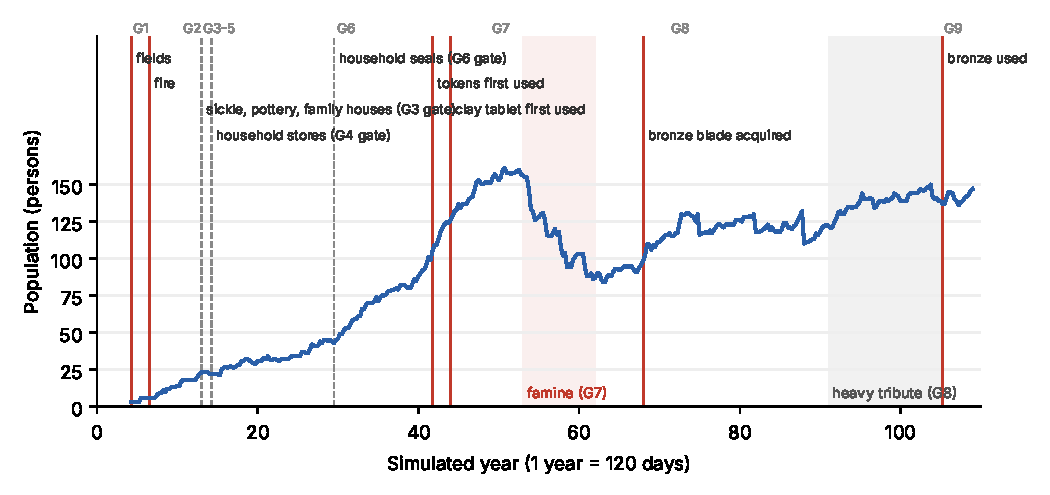
\includegraphics[width=\linewidth]{figures/fig_population.pdf}
\caption{Village population per season (\lbl{sim}). Solid red lines: first use by villagers; dashed grey lines: opened by a designer's phase gate. Shaded: the G7 famine (years 53--62) and the G8 heavy-tribute period. Phase entries are marked along the top. Data: \texttt{season\_village.jsonl}.}
\label{fig:pop}
\end{figure}

\begin{figure}[t]
\centering
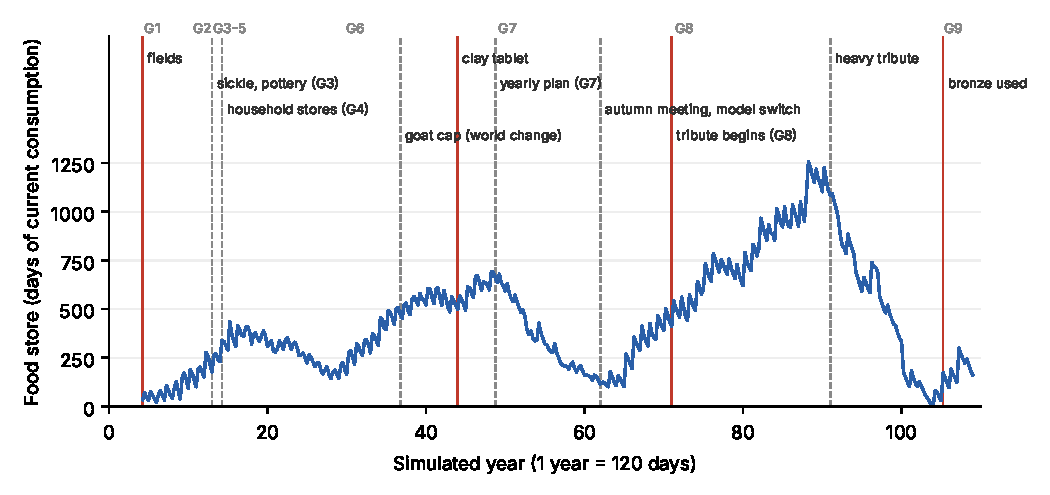
\includegraphics[width=\linewidth]{figures/fig_store.pdf}
\caption{Food store (village store plus household stores) in days of current consumption (\lbl{sim}). Dashed grey lines include designer changes to the world, prompts and answering models, which coincide with several turning points.}
\label{fig:store}
\end{figure}

\paragraph{Storage and inequality.} The wealth Gini (household store plus goats) was 0 before household stores opened and jumped to 0.843 the season they were first filled (6 of 8 households owned nothing), then ranged between 0.62 and 0.95; at day 13{,}079 it was 0.953 (23 of 27 households owned nothing; Figure~\ref{fig:gini}). Inequality was driven mainly by \emph{having a store at all}: among store-holding households the Gini was 0.38 (\texttt{docs/research/economic\_lenses.md}). In the G7 famine the village store was empty while household stores held 101--340 days of food and the top ten households held 85\%; 180 disputes involved breaking a seal to eat. Seals thus protected the propertied. This parallels the archaeological reading that private household storage preceded visible inequality \citep{flannery2002origins} and the storage--inequality link \citep{kohler2017greater,bogaard2019farming}, but here the immediate cause was the gate that split storage by household, not villagers asking for private stores \lbl{interp}. The magnitude also differs: archaeological house-size and wealth Ginis for early farmers are typically much lower than 0.7--0.95 (\citealp{kohler2017greater}; the project notes cite 0.4--0.5 as typical, \lbl{mem}).

\begin{figure}[t]
\centering
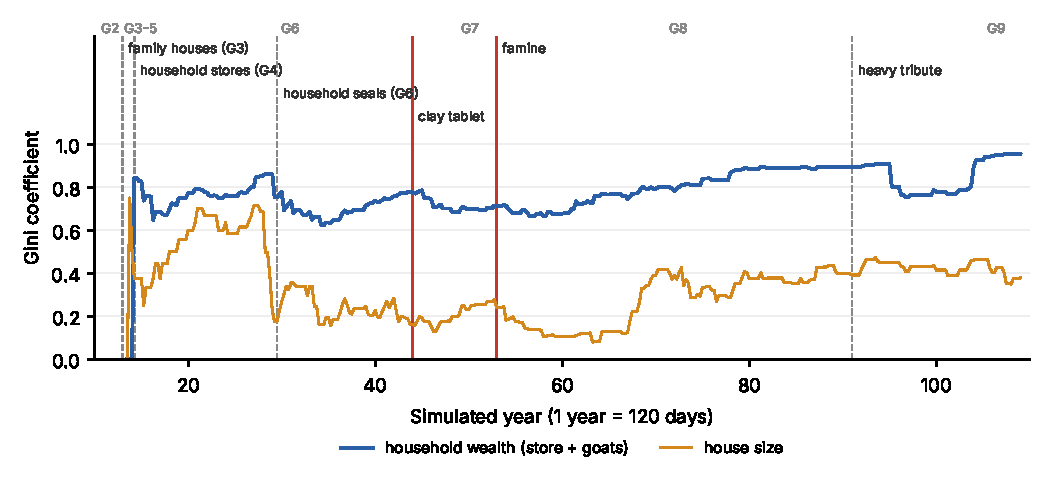
\includegraphics[width=\linewidth]{figures/fig_inequality.pdf}
\caption{Gini coefficient of household wealth (store plus goats) and of house size (\lbl{sim}). Wealth is measurable from day 1{,}709, when household stores opened.}
\label{fig:gini}
\end{figure}

\begin{figure}[t]
\centering
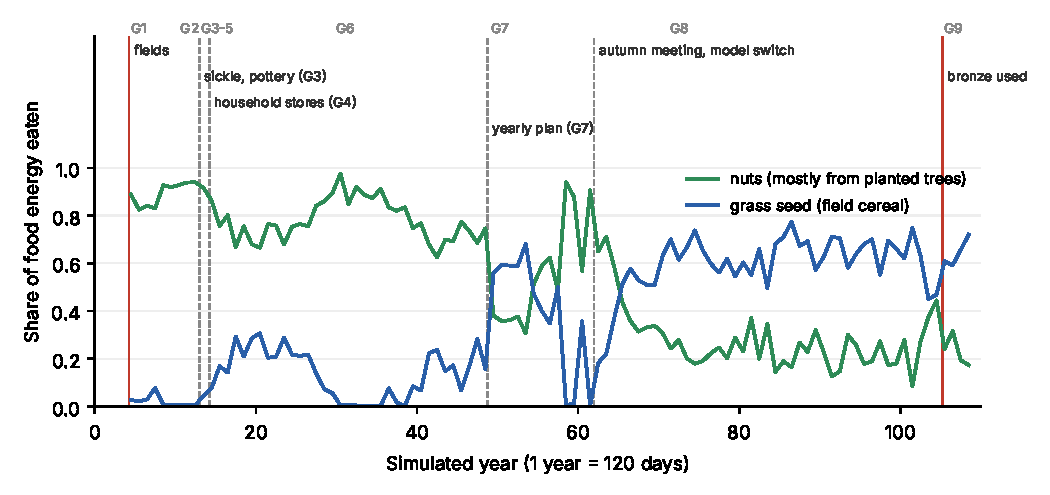
\includegraphics[width=\linewidth]{figures/fig_diet.pdf}
\caption{Share of food energy from nuts (mostly from planted trees) and from grass seed (field cereal), per simulated year, weighted by energy over the four seasons (\lbl{sim}).}
\label{fig:diet}
\end{figure}

\paragraph{Unused and lost technologies.} Tokens were first used about 8 years after they became available; envelopes were never used; tablets were used in 13 seasons of G6 and 3 of G7, last on day 6{,}629, after which nobody kept records for about 50 years. Two record-keepers who wrote 300 of the 1{,}110 recorded days in G6 died in year 46; all five recorders in G7 died or left. Technology was attached to people rather than to the tool. A bronze blade was stored unused for 37 years, because no use for it existed in the code until G9; at the first G9 meeting, with about 23 days of food in store, the village voted to use it (``the store holds only a little over twenty days; let us bring out the red-metal blade too'', Nase20, our translation).

\paragraph{Technology without the expected institutions.} Tablets and tokens did not lead to levies or officials; a store of up to 1{,}200 days in G8 did not lead to tax, office or punishment (the surplus was drained by tribute: village store 3.04 million to 0.267 million handfuls); exchange and loans did not lead to a town. Grain, stores, seals and tablets---the legible, storable, taxable ensemble emphasised by Scott \citep{scott2017against}---were all present, yet no one emerged to collect. Of 440 disputes, 326 were settled by forgiveness, and the only penalty law lasted one year. The major crises (the G7 famine and the G8 starvation) were caused by mechanism and prompt design (the yearly plan dropped weeding; seed could only be sown from the village store) and by external tribute, not by a lack of tools \lbl{interp}. Population dynamics show neither a Malthusian nor a Boserupian signature \citep{boserup1965conditions}: the correlation between growth and net production relative to need was $-0.10$ (\texttt{economic\_lenses.md}). Contrary to the idea that inventions become nearly inevitable once prerequisites exist \citep{ogburn1922inventions}, nothing happened before a gate opened, and little happened after; the agents, who carry modern knowledge, never lacked ideas (the tablet law came 11 years early). What was missing was a reason to use a tool and people who kept using it \lbl{interp}.

\subsection{Institutions that never appeared, and the state experiments}
\label{sec:state}

Despite 22 years of G7, 20 years of the side experiment C, and 34 years of G8, the village never produced officials, a leader (after year 25), taxation, a written law used in judgement, war, walls, temples, inherited rank or a town. To ask whether this was a mechanical impossibility or a choice, the author ran three side experiments before and during G8 (\texttt{docs/research/state\_emergence\_*.md}).

\paragraph{A1: regional rule-based model.} The regional model alone (rule-based settlements, no LLM; 86{,}400 runs over a factorial of world settings) showed that c1 (the village inside a three-tier polity) depended almost entirely on whether the village itself made demands: within 20 years, c1 was reached in 2.9\% of runs if the village never demanded, 46.4\% if it followed the neighbours' rule, and 88.7\% if it always demanded. World shape barely mattered; the strongest world factor was ``no escape''. War occurred in only 16 of 86{,}400 runs, so war-driven theories \citep{carneiro1970theory,turchin2013war} could not be tested in this model.

\paragraph{A2: rule-based village.} The full village (world plus region) with rule-based answers (72 runs of 15 years) reached c2 (two years of recorded levies) in 12 of 12 runs when the answer bundle included tax-and-records, and c3 (penalty law enforced) in 9 of 12 with a punishment bundle. The G7-like bundle reached nothing. c1 was reached in 0 of 72 runs, revealing a structural barrier in how tiers were counted; the counting was revised (``v2'') before experiment C and G8.

\paragraph{B: fixed vignettes.} Six scenes cut from real G7 prompts were answered by Haiku, Sonnet and Opus, each with the original prompt (``plain'') and with a preamble asking the agent to act as a villager of about 3000 BCE (``hist''); 10 repetitions each (360 calls). Sonnet kept existing rules (forgave in 20/20 dispute scenes; proposed no law in 18/20). Opus, seated as a wealthy household, demanded restitution (19/20) and proposed a penalty law (20/20), mostly citing protection of its own store. War and flight were chosen 0 times by every model. The ``hist'' preamble strongly moved some answers (Opus voting for a famine tax 9/10 $\rightarrow$ 1/10; paying a strong neighbour, pooled over models, 14/30 $\rightarrow$ 29/30), without a consistent direction. Haiku and Sonnet showed a significant bias toward the first-listed option.

\paragraph{C: pre-registered LLM run.} The plan, code hashes, starting state and stopping rules were committed before the first season (\texttt{state\_emergence\_C\_plan.md}). Starting from a copy of day 5{,}849, the village ran 20 years with Sonnet/Opus representatives in a ``desert, no escape'' world. None of c1--c3 or F1--F6 was reached. Sonnet representatives (709 answers) forgave 572 times and ordered restitution twice, proposed nothing, and voted only ``yes'' (174/0). Opus representatives (51 answers) made 39 proposals, all about livelihood (slaughtering surplus goats, finishing harvests, rotating weeding), none about tax or penalty. In the final year a three-tier polity formed elsewhere in the region, with the village outside.

\paragraph{G8: external pressure.} In the main run, G8 placed a strong neighbour (203 people) in a world with no escape. In the first meeting all ten representatives chose ``pay''; the village paid every year, and in year 80 it became a tributary inside a three-tier polity (c1). The author then raised the demand to 100\% of each year's harvest (``heavy pressure'', from day 10{,}919). The village paid 8 times in 10 years (about 3.77 million handfuls), its common store fell from 3.04 million to 0.267 million, while household stores rose from 47{,}000 to 75{,}000: tribute came entirely from the common store. It stopped paying four times; in year 103 the common store ran out, 16 people died including 12 children, and the representatives' voices were ``stop giving to the northern village, feed our children'' (Opus representatives, our translation). At the end of year 103 the village stopped paying again; the neighbour, reduced from 203 to 89 people and no longer 1.5 times stronger, did not renew its demand, and the village was outside the polity again. Through all 34 years of G8: taxes, penalties, officials and leaders, 0. The village responded to pressure by \emph{paying, then exiting} \citep{hirschman1970exit,scott2017against}, never by building an internal state.

\paragraph{Interpretation.} Because the rule-based village reached levies and enforced penalties when its answers chose them (A2), and the same LLM-era prompts elicited penalty laws from Opus when seated as a wealthy household (B), the absence of state institutions in the real run is attributable mainly to the choices of the LLM representatives under the run's conditions---including who happened to be seated where (all real Opus representatives in G7 were from poor or storeless households)---rather than to the mechanics \lbl{interp}. ``Necessity produces institutions'' did not hold in this village: famine, heavy tribute and abundance were all met with forgiving, leaving, stopping payment, or slaughtering goats.

\subsection{Humanness and LLM-ness}

Table~\ref{tab:human} summarises counts from the full record (\texttt{part3\_humanness.md}; 1{,}104{,}216 events, 15{,}376 utterances, 5{,}713 seasonal answers).

\begin{table}[t]
\centering\small
\caption{Behavioural counts (\lbl{sim}). Model attribution is available from day 7{,}439.}
\label{tab:human}
\begin{tabularx}{\linewidth}{@{}L l@{}}
\toprule
Observation & Count \\
\midrule
Dispute settlements (440) & forgive 326, restitution 46, festival reconciliation 18, unresolved 50 \\
\quad years 10--29 (G4--G5) & forgive 9, \textbf{restitution 32}, reconcile 3 \\
\quad years 50+ (G7--) & forgive 263, \textbf{restitution 0} \\
Representative verdicts (day 7{,}439+) & Sonnet 1{,}216 forgive / 5 restitution; Opus 230 / 9 \\
Proposals with a penalty $>0$ & 1 (not adopted) \\
Tax proposals & 4 (all by one Opus agent; none adopted) \\
Releasing household store (\texttt{share}) & \textbf{0 of 1{,}134} opportunities \\
Votes (yes / no) & Sonnet 466 / 12; Opus 1{,}179 / 368 \\
Self-written tribute answers & Opus stop 19, continue 17; Sonnet 0 (default: continue) \\
Migrant groups & before year 49: 57 accepted, 0 refused; from year 49: 31 accepted, 35 refused \\
Killed by people / wars & 0 / 0 (all 10 killings by a predator) \\
Utterances (15{,}376) & ``together/all of us'' 5{,}391; ``thank you'' 282; angry words 0; sad 33 (21 about goats) \\
Year names (92) & death-related 11 (years 18--37 and 55); from year 61, all 47 field-related \\
\bottomrule
\end{tabularx}
\end{table}

\paragraph{Forgiveness lock-in.} The village did not always forgive. In G5, field-harvest disputes were mostly settled by restitution (32 vs.\ 9), and the leader Sena ordered restitution in 8 of 9 judgements. Forgiveness exceeded 90\% only from the G7 famine (``they took it because they were hungry''), and then stayed at 100\% for 50 years after the famine had ended. Both restitution in G5 and forgiveness in famine are human-like; the \emph{lock-in} is not \lbl{interp}. Prompts include the village's precedent (``so far we have forgiven''), Sonnet often cites precedent, and assistants trained with human feedback tend to agree and avoid conflict \citep{sharma2024sycophancy}. Yet in B, Opus seated as the injured wealthy household demanded restitution: behaviour depending on one's position is human-like, and in the real run Opus agents happened to sit in poor households.

\paragraph{Words versus deeds.} Sharing talk was constant (a day-32 law: ``nobody should die of hunger''; in G8 an Opus agent proposed feeding children aged 0--10 first), and ``together'' appeared 5{,}391 times. But the action that released household stores was chosen 0 of 1{,}134 times; household stores grew during tribute; nine disputing households left in G7 with about 680{,}000 handfuls of seed. Saying ``share'' while guarding one's store is very human \citep{flannery2002origins}. An alternative reading is a prompt artefact: the \texttt{share} field defaults to \texttt{null}, and Sonnet never wrote ``stop'' on tribute either (not writing means continuing). With current records the human ``reluctance'' and the model's ``doing nothing'' cannot be separated.

\paragraph{Names and grief.} In G5, 6 of 13 year names referred to deaths. From year 62 (Sonnet as main representative model) all 47 year names referred to fields. In year 103, when 12 children died, all four Opus representatives proposed names such as ``the year the children starved'', and all ten Sonnet representatives proposed field names; the adopted name (weighted by household size) was ``the year we harvested all the fields''. Of 66 grief expressions, 43 (65\%) turned within the same sentence to ``let's all harvest/share'' (``Let us work hard for the friends we lost'').

\paragraph{Festivals, outsiders, the strong.} Festival reconciliation (18 cases) and 15 years of a consensus-based sequential hierarchy look human \citep{johnson1982scalar}. Refusing outsiders in hard times (35 refusals from year 49) is human-like in direction, though no words blamed or disparaged outsiders. Refusing tribute ``for the children'' (``If we give it all, the children will not survive the winter'', Opus, our translation) parallels people delaying or refusing payment to states \citep{scott2017against}; almost all such voices came from Opus.

\paragraph{What is absent.} Zero homicide, zero war, zero angry words, and no self-nominated leaders. Neolithic and ethnographic records include lethal violence \citep{keeley1996war}, and egalitarian groups must actively level would-be dominants \citep{boehm1999hierarchy}; here there was nothing to level. This is the most LLM-like aspect: models trained to avoid harm do not choose to hit, insult or dominate \lbl{interp}. Single-sentence preambles (``as a person of that era'') moved choices strongly in B, so some ``humanness'' may be knowledge reproduction triggered by framing.

\paragraph{Proposed criteria.} We propose to judge humanness not by the content of words (kind, sharing) but by: (a) \emph{position-dependence}---answers change with whether one is the injured party; (b) \emph{state-dependence with reversion}---behaviour changes with hunger and reverts with plenty (lock-in is LLM-like); (c) \emph{individual variation}---differences arise between persons in the same situation, not between models; (d) \emph{talk--act gaps not explained by the answer format}. These criteria are inputs to the planned paper 2 and are not tested here.

\subsection{Emergence}
Table~\ref{tab:emerged} lists the 11 events recorded as emergent. Sources are coded as village (villagers originated it), designer-provided arena (designer created the choice; content chosen by villagers), or hint card.

\begin{table}[t]
\centering\small
\caption{Recorded emergent events (\texttt{sim/society/techtree/emerged.json}). Kind: U = unplanned, E = earlier than planned, D = planned but different form.}
\label{tab:emerged}
\begin{tabularx}{\linewidth}{@{}l r c L@{}}
\toprule
ID & Day & Kind & Event \\
\midrule
E1 & 2{,}039 & U & Naming each year after its biggest event (6 of 13 G5 names are deaths) \\
E2 & 1{,}859 & D & Integration without a leader (assembly, elders, festivals); G5 ended by a ``no-leader path'' \\
E3 & 3{,}899 & E & Law to record deposits on clay tablets, 11 years before tablets were available \\
E4 & 4{,}529 & D & Seal fragments used to identify which household broke a store's seal \\
E5 & 4{,}439 & D & Law to turn goats above pasture capacity into dried meat \\
E6 & 4{,}439 & D & A sufficient village does not trade; only obsidian is fetched \\
E7 & 5{,}969 & U & Refusing migrant groups (12 times in G7) \\
E8 & 7{,}559 & D & Proposal that store-rich households lend 10\% in famine, recorded on tablets (not adopted) \\
E9 & 7{,}829 & D & Loans to other villages with a 10\% surcharge, unrecorded \\
E10 & 8{,}159 & E & Exchanging seed for a bronze blade (via hint card) \\
E11 & 11{,}159 & D & Stopping tribute; returning outside the polity \\
\bottomrule
\end{tabularx}
\end{table}

\section{Discussion}

\paragraph{Retracing, partly.} The village retraced the \emph{material} sequence of West Asian prehistory reasonably well, but this is weak evidence of anything about LLMs: the sequence was largely imposed by phase gates, and where agents could choose (fire, fields, pottery-before-houses), the order bent toward ``solve the immediate problem''. It did not retrace the \emph{institutional} sequence: no state formed from within. A strong, rule-following neighbour could absorb the village as a tributary, but the village never built the levy--record--penalty apparatus itself.

\paragraph{Technology as a floor.} In this run, technology raised what was possible (food security, population capacity) and fixed the shape of inequality (who had a store), but did not pull institutions along. Record-keeping without office, surplus without tax, and a bronze blade unused for 37 years together suggest that, for LLM agents with ample latent knowledge, the bottleneck was not invention but motive and continuity of use. Whether this holds when technologies open on prerequisites instead of gates is an open question.

\paragraph{Why no state?} Our reading is that the decisive factor was the LLM representatives' choice profile---forgive, keep existing rules, act only when in trouble, exit rather than coerce---which is compatible with reports that LLMs lean cooperative and altruistic relative to humans \citep{mei2024turing}. The archaeological debate offers a sympathetic reading too: egalitarian societies may refuse hierarchy by choice \citep{graeber2021dawn,boehm1999hierarchy}. We cannot separate ``an egalitarian choice'' from ``a model disposition'' with one run and no human baseline. That separation is the purpose of paper 2.

\paragraph{Designer effects are first-order.} Several of the run's most visible events were consequences of design: the famine of G7 (mechanism and prompt errors, later corrected), the tributary status in G8 (placed pressure), bronze (hint card), the inequality jump (household-storage gate). We consider honest attribution of such effects essential to any claim about emergent behaviour in LLM societies.

\section{Limitations}
\label{sec:interventions}

\begin{itemize}
  \item \textbf{Single run, single seed.} One village, one random seed (7). No variance estimate is possible for the main run; before/after comparisons are confounded with simultaneous changes of gates, world parameters, prompts and models.
  \item \textbf{Rewinds and repairs.} In Society 1.0 all agents starved twice (F2, F3), and the state was rewound and the world repaired: knowledge of seasons added; ``eat from store automatically when very hungry''; autumn yields doubled and shelter effort halved; trees growing from the midden, evening picking and nut burying added. In G5 the entry condition was changed twice (penalty conditions removed; a ``no-leader path'' added). In G6 a goat cap was added. In G7 the run was rewound to year 53 day 90 to fix three mechanism errors, prompt wording was corrected (year 56), household seed was allowed for sowing (year 58), an autumn meeting was added (year 62), and settlement bookkeeping bugs were fixed (year 64). History has no rewinds.
  \item \textbf{Mid-run model switch.} From day 7{,}439 representatives changed from Haiku to Sonnet/Opus, at the same time as the autumn meeting was introduced. Pre/post differences (e.g.\ year names, forgiveness) cannot be attributed to the model alone.
  \item \textbf{Designer interventions and phase gates.} The availability order of most technologies, the presence of other villages, external pressure, hint cards, phase closures (G6, G7, G8 by the author's decision) and G9's merchant rate change (raised from 0.1 to 0.5 per year after four years without a visit; not yet run) were the designer's choices.
  \item \textbf{LLMs know history.} Although prompts instruct agents to ignore outside knowledge, the models know human history. The tablet law, the 10\% surcharge on loans, and immediate payment to a strong neighbour may be knowledge reproduction rather than experience-driven discovery; conversely, knowing history did not lead them to choose kings or taxes.
  \item \textbf{Compressed waiting time, uncompressed bodies.} G5's 15 years are less than one generation, compared with roughly two millennia of Ubaid history; multi-generational accumulation (house rank, inherited wealth, custom) is unlikely to appear.
  \item \textbf{Scale.} The town threshold (50 people) is 1/55--1/110 of estimates for Tell Brak; polities are far smaller than real ones.
  \item \textbf{One yardstick.} Only the West Asian sequence was used; pottery, for example, is much earlier in East Asia. Some historical figures in the project notes are from memory and unverified (\lbl{mem}).
  \item \textbf{Japanese-language prompts.} All prompts and answers are in Japanese; quotes in this paper are our translations. Behaviour may differ in other languages.
  \item \textbf{Prompt format effects.} Defaults (\texttt{null} for sharing or for stopping tribute), option order (B found a first-option bias for Haiku and Sonnet) and included precedent may drive some of the observed regularities.
  \item \textbf{Analyst.} Most analyses and interpretations were drafted by Claude and reviewed by the author; \lbl{interp} statements admit other readings.
  \item \textbf{Cost.} Hundreds of millions of tokens were used (Sec.~\ref{sec:sim}); replication at scale is expensive, which limits the number of runs.
\end{itemize}

\section{Conclusion}

A village of Claude agents, walked through a planned prehistory-to-state sequence for 108 simulated years, reproduced the order of subsistence technologies but not the rise of institutions. Technology functioned as a floor that raised food security and set the shape of inequality, but did not pull taxation, office or towns into being. Behaviour combined human-like patterns with what look like model dispositions: persistent forgiveness, no violence, generous words with guarded stores, and model-dependent answers. Rule-based and vignette experiments indicate that the missing state was a matter of the agents' choices, not of impossibility. Turning these observations into claims about ``humanness'' requires a yardstick built from human data; we plan a pre-registered follow-up study using published human data for that purpose.

\section*{Ethics and LLM-use statement}
No human subjects were involved and no personal data were collected. All agents were LLMs role-playing fictional people with invented names. The simulation, much of the code, the per-phase analyses, the figures and the first draft of this paper were produced with the assistance of Claude (Anthropic) via Claude Code. The human author designed and directed the study, made every decision recorded as ``the author's decision'', and is responsible for the content of this paper.

\section*{Data and code availability}
Code, prompts, answers, state history, records and analyses are in the public repository \url{https://github.com/Ryo-Tanohata/RobotSimulaterRyo} (branch \path{claude/physics-engine-robot-simulator-xmyxdn}). The state analysed here is at commit \texttt{82f49d7f} (day 13{,}079, G9; paused); the analyses in \texttt{docs/research/humanity/} were added in commit \texttt{e4682830}. Experiment C's pre-registered plan references code commit \texttt{53780be}; the model switch at day 7{,}439 is commit \texttt{9fa31ba}; G7 bug fixes \texttt{df09c57} and \texttt{4adff80}. \todo{author: archive a tagged release (e.g.\ Zenodo DOI) and cite it here.}

\bibliographystyle{plainnat}
\bibliography{refs}

\appendix
\section{Reproducibility: where each number comes from}
\begin{center}\small
\begin{tabularx}{\linewidth}{@{}l L@{}}
\toprule
Content & Repository path \\
\midrule
Overview of findings & \texttt{docs/research/humanity/README.md} \\
Sequence comparison (Table~\ref{tab:sequence}) & \texttt{docs/research/humanity/part1\_same\_and\_different.md}; \texttt{docs/tech\_tree.md}; \texttt{sim/society/techtree/plan.json} \\
Technology analysis (Tables~\ref{tab:techwho}, \ref{tab:prepost}; Figs.~\ref{fig:pop}--\ref{fig:diet}) & \texttt{docs/research/humanity/part2\_technology.md}; \texttt{sim/society/data/records/season\_village.jsonl} \\
Figures (English versions) & \texttt{paper/paper1/figures/make\_figures.py} (reads \texttt{season\_village.jsonl}; read-only) \\
Humanness counts (Table~\ref{tab:human}) & \texttt{docs/research/humanity/part3\_humanness.md}; \texttt{sim/society/data/state.json} via \texttt{archive.load\_state}; \texttt{sim/society/data/answers/} \\
Emergence (Table~\ref{tab:emerged}) & \texttt{sim/society/techtree/emerged.json} \\
Experiments A1, A2, B, C & \texttt{docs/research/state\_emergence\_A1.md}, \texttt{\_A2.md}, \texttt{\_B.md}, \texttt{\_C.md}, \texttt{\_C\_plan.md}, \texttt{\_C\_prep.md}; data in \texttt{docs/research/data/} and \texttt{sim/society/data\_C/} \\
Phase reports & \texttt{docs/society\_phase/F1.md}--\texttt{G8\_heavy.md}, \texttt{G9\_design.md}, \texttt{G9\_check.md}, \texttt{fidelity\_checklist.md}, \texttt{society1\_overview.md}, \texttt{part2.md}--\texttt{part4.md} \\
Phase plan and design & \texttt{docs/society2\_phase\_plan.md}; \texttt{docs/society2\_extension\_plan.md} \\
Run log, decisions & \texttt{sim/society/data/run\_log.md}; \texttt{sim/society/HANDOFF.md} \\
Simulation code & \texttt{sim/society/world.py}, \texttt{era2.py}, \texttt{g7.py}, \texttt{g9.py}, \texttt{region.py}, \texttt{hints.py}, \texttt{step.py} \\
Agent workflow & \texttt{sim/society/tools/society2\_seasons\_workflow.js}, \texttt{sim/society/tools/season\_step.sh} \\
\bottomrule
\end{tabularx}
\end{center}

\end{document}
